\chapter{\label{chap:chap5}{Research Methodology}}

Due to the empirical nature of our objectives shown in Chapter \ref{chap:chap3}, this research aims to create or adapt an inspection review technique to guide the quality evaluation of BDD scenarios and enhance software development team's knowledge on how good are they. 

Before knowing how to reach that goal and build a proper research design, we gathered information that would improve our grasp on the main concepts involved with the quality of BDD scenarios in order to help us better define our research problem and suggest hypotheses. That approach had lead us to a better understanding of requirements quality and different formats of acceptance tests. With the possession of that knowledge, summarized in Chapter \ref{chap:chap4}, we are now able to know what requirements quality attributes exists, how they are measured (through some common reading techniques) and from which other formats BDD could borrow those characteristics from. This understanding also helped us create this research plan. This is what we called Phase 1 on our research design shown in Figure \ref{fig:design}

\begin{figure}[h!]
\centering
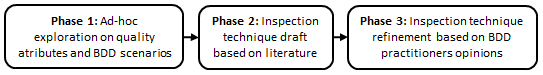
\includegraphics[scale=0.9]{images/Research-Plan}
\caption{Research Design}
\label{fig:design}
\end{figure}

\begin{table}[!b]
\renewcommand{\arraystretch}{1.3}
\caption{Research Choices}
\label{tbl:research_design}
\centering
\begin{tabular}{|m{6cm}|m{6cm}|}
\hline
 \textbf{Research Design} & qualitative\\
 \hline
 \textbf{Strategy of Inquiry} & grounded theory\\
 \hline
 \textbf{Data Collection Type} & interviews\\
\hline
\end{tabular}
\end{table}

Since there is no standard on what is considered a "good" scenario due to the few views on this matter, this is a concept that still needs to be fully understood. A qualitative approach is suitable for situations like this, as mentioned by \cite{Creswell_2008}. In order to develop a technique that would help practitioners judge the quality of BDD scenarios, we first need to know what characteristics could define "good" scenarios and how they could be measured (represented on Phase 2 of our research design in Figure \ref{fig:design}) and match them with the opinion of industry practitioners to clarify if they are really important when writing those scenarios - or even if other characteristics or measurements should be also worth mentioning (represented on Phase 3 of our research design in Figure \ref{fig:design}). As the views of the participants will deliver us an abstract theory about how they perceive "good" scenarios, our strategy of inquiry will be based on grounded theory \cite{Creswell_2008}. Table \ref{tbl:research_design} summarizes our research choices.